%!TEX root = bachelor_thesis.tex

\chapter{Entdeckung und Namensgebung}
\label{chapter-kapitel1}

Historisch bezeichnete der Begriff kosmische Radioquellen, die in den 1950er Jahren nicht als Radiogalaxien identifiziert werden konnten, sondern in optischen Beobachtungen blau und „sternförmig“ (also nicht flächig) erschienen. 1963 stellte Maarten Schmidt fest, dass die Radioquelle 3C 273 kein naher Stern ist, sondern mit einer Rotverschiebung von 0,158 im Bereich ferner Galaxien liegt, also nur \textit{quasi} sternartig ist. Spätere Beobachtungen zeigten, dass die hellen sternartigen Quasare doch in die Kerne von Galaxien eingebettet sind, die aber wegen der großen Entfernung schwach erscheinen. Durch die starke Rotverschiebung aufgrund der Expansion des Universums wurden Quasare als sehr weit entfernte Objekte erkannt. Diese Folgerung konnte seit der Entdeckung von Gravitationslinsen unabhängig bestätigt werden. Quasare wurden inzwischen bis zu einer Rotverschiebung von 7,1 entdeckt.

\begin{figure}[h]
	\centering
	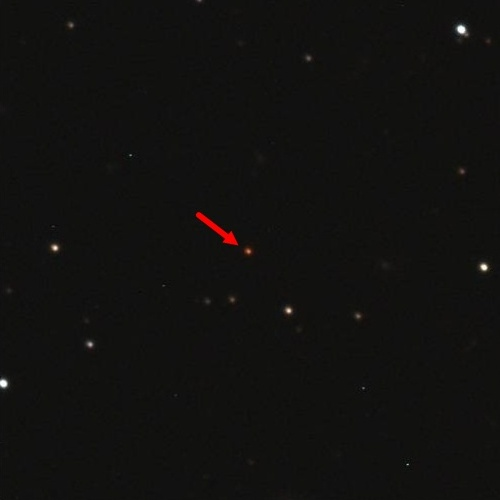
\includegraphics[width=5cm]{Imgs/QSO_APM_08279+5225_marked}
	\caption{Fotografische Aufnahme des Quasars APM08279+5225\\\hspace*{3cm}(Rotverschiebung z=3,9)\cite{wikiQuasar2}}
	\label{fig:darstQuasar}
\end{figure}

Mit der im Jahr 2010 gemachten Entdeckung, dass der 1,6 Mrd. Lichtjahre entfernte Quasar SDSS J0013+1523 als Gravitationslinse für eine 5,9 Mrd. Lichtjahre dahinter liegende Galaxie wirkt, ergibt sich eine direkte Möglichkeit zur Massenbestimmung eines Quasars.[1][2]

Die Bezeichnung \textit{QSO (quasi-stellar object)} schließt nicht nur die klassischen \textit{radiolauten} Quasare ein, sondern auch \textit{radioleise} Objekte mit schwacher Radioemission, aber sonst ähnlichen Eigenschaften. Häufig wird aber der Begriff Quasar etwas ungenau für beide Klassen benutzt.